% -------------------------------
% --- PREAMBLE ---
% -------------------------------
\documentclass[a4paper,11pt]{article}
\usepackage[utf8]{inputenc}

\usepackage[T1]{fontenc}
\usepackage[swedish]{babel}

\usepackage{array,longtable}
\usepackage{amsmath,amssymb,amsfonts,amsthm}    % Typical maths resource packages
\usepackage{graphicx}                           % Packages to allow inclusion of graphics
%\usepackage[authoryear]{natbib}                 % literature reference style
\usepackage{natbib}
\usepackage[bf]{caption}
\usepackage{textcomp}                           % For single quotes
\usepackage{floatrow}                           % For image and table position
\usepackage{booktabs}                           % For tables
\usepackage[hidelinks]{hyperref}
% \usepackage[colorlinks=true]{hyperref}
% \usepackage[bottom]{footmisc}
\usepackage[bottom, flushmargin]{footmisc}                   % For footnotes
%\usepackage[citebordercolor={0 1 0}]{hyperref}                           % For creating hyperlinks in cross references
\usepackage{footnotebackref}

% From {rticles}
\newlength{\csllabelwidth}
\setlength{\csllabelwidth}{3em}
\newlength{\cslhangindent}
\setlength{\cslhangindent}{1.5em}
% for Pandoc 2.8 to 2.10.1
\newenvironment{cslreferences}%
  {}%
  {\par}
% For Pandoc 2.11+
% As noted by @mirh [2] is needed instead of [3] for 2.12
\newenvironment{CSLReferences}[2] % #1 hanging-ident, #2 entry spacing
 {% don't indent paragraphs
  \setlength{\parindent}{0pt}
  % turn on hanging indent if param 1 is 1
  \ifodd #1 \everypar{\setlength{\hangindent}{\cslhangindent}}\ignorespaces\fi
  % set entry spacing
  \ifnum #2 > 0
  \setlength{\parskip}{#2\baselineskip}
  \fi
 }%
 {}
\usepackage{calc} % for calculating minipage widths
\newcommand{\CSLBlock}[1]{#1\hfill\break}
\newcommand{\CSLLeftMargin}[1]{\parbox[t]{\csllabelwidth}{#1}}
\newcommand{\CSLRightInline}[1]{\parbox[t]{\linewidth - \csllabelwidth}{#1}}
\newcommand{\CSLIndent}[1]{\hspace{\cslhangindent}#1}


% -------------------------------
% --- some layout definitions ---
% -------------------------------

% define topline
\usepackage[automark]{scrlayer-scrpage}
\pagestyle{scrheadings}
\automark{section}
\clearscrheadings
\ohead{\headmark}

% define citation style
\bibliographystyle{apalike}

% define page size, margin size
\setlength{\headheight}{1.1\baselineskip}
\voffset=-2cm
\hoffset=-3cm
\textheight24cm
\textwidth15.5cm
\topmargin1cm
\oddsidemargin3cm
\evensidemargin3cm
\setcounter{secnumdepth}{3}
\setcounter{tocdepth}{3}
  \usepackage[parfill]{parskip}

% define line spacing = 1.5
\renewcommand{\baselinestretch}{1.5}

% define position of graphics
\floatsetup[figure]{capposition=bottom}
\floatsetup[table]{capposition=bottom}
\floatplacement{figure}{tb}
\floatplacement{table}{tb}

% save thesis parameters for later
\newcommand{\thesisauthor}{Inge Tabell}
\newcommand{\thesisdate}{}

% define tightlist to work with newer versions of pandoc
\providecommand{\tightlist}{%
  \setlength{\itemsep}{0pt}\setlength{\parskip}{0pt}}

% change spacing
\setlength {\parskip}{1em}

% Additional LaTeX parameters added in the YAML header of index.Rmd

% --------------------------------------
% --------------------------------------
% --------------------------------------
% --- the structure the tex document ---
% ---  (this our recommendation) -------
% frontmatter:
%   - titlepage (mandatory),
%   - acknowledgement,
%   - abstract,
%   - table of contents (mandatory),
%   - list of abbreviations (not mandatory),
%   - list of figures (not mandatory),
%   - list of tables  (not mandatory) .
%
% body of the thesis (the structure of the thesis body is not mandatory, but the list of literature is mandatory):
%   - introduction,
%   - methods,
%   - data,
%   - results,
%   - conclusion,
%   - literature (mandatory),
%   - appendix (figures, tables).
%
% last page:
%   - declaration of authorship (mandatory).
% --------------------------------------
% --------------------------------------
% --------------------------------------
\begin{document}
% -------------------------------
% --- frontmatter: Swedish title page ---
% -------------------------------
\thispagestyle{empty}
\begin{center}

\includegraphics[width=7cm]{UU_logo_CMYK.eps}
\end{center}
\vspace{1.5cm}
\begin{center}
\begin{Large}
{\bf UPPSATSENS TITEL}
\end{Large}
\end{center}
\vskip1.5cm
\renewcommand{\baselinestretch}{1}
\begin{center}
{\large Inge Tabell}
\vskip2.5cm
\begin{center}
\begin{large}
{\it Kanditatuppsats i statistik}\\
\end{large}
\end{center}
\vskip2cm
{\large\it Handledare}\\
{\large Efraim Stolle}
\vskip2cm
{\large 20yy}
\end{center}\vfill

% ------------------------------------
% --- frontmatter: Acknowledgement ---
% ------------------------------------
\newpage
\hypertarget{fuxf6rfattarens-tack}{%
\section*{Författarens tack}\label{fuxf6rfattarens-tack}}
\addcontentsline{toc}{section}{Författarens tack}

I want to thank a few people.
\pagestyle{plain}
\pagenumbering{roman}   % define page number in roman style
\setcounter{page}{1}    % start page numbering

% -----------------------------
% --- frontmatter: Abstract ---
% -----------------------------
\newpage
\hypertarget{sammanfattning}{%
\section*{Sammanfattning}\label{sammanfattning}}
\addcontentsline{toc}{section}{Sammanfattning}

A clearly worded, short, precise, abstract of no more than 300 Words; No formulas; Avoid references utmost; Same tense; No indentation or enumeration etc.; Write in normal text (no italic, bold or underline)

% -----------------------------
% --- frontmatter: Contents ---
% -----------------------------
\newpage
\tableofcontents
\clearpage

% ----------------------------------------------------------
% --- frontmatter: List of Abbreviations (not mandatory) ---
% ----------------------------------------------------------
\newpage
\hypertarget{fuxf6rkortningar}{%
\section*{Förkortningar}\label{fuxf6rkortningar}}
\addcontentsline{toc}{section}{Förkortningar}
\begin{tabular}{rp{0.2cm}lp{1cm}rp{0.2cm}l}
    CPI     & &  Consumer Price Index   & & ETF     & &  Equity Traded Funds  \\
    ETH     & &  Eat the Horse          & & XLM     & &  Xetra Liquidity
\end{tabular}
% ----------------------------------------------------
% --- frontmatter: List of Figures (not mandatory) ---
% ----------------------------------------------------
\newpage
\listoffigures
\addcontentsline{toc}{section}{Figurer}

% ---------------------------------------------------
% --- frontmatter: List of Tables (not mandatory) ---
% ---------------------------------------------------
\newpage
\listoftables
\addcontentsline{toc}{section}{Tabeller}

% -------------------------------
% --- main body of the thesis ---
% -------------------------------
\newpage
\pagestyle{plain}
\setcounter{page}{1}    % start page numbering anew
\pagenumbering{arabic}  % page numbers in arabic style

\hypertarget{about-this-thesis-template}{%
\section*{About this Thesis Template}\label{about-this-thesis-template}}
\addcontentsline{toc}{section}{About this Thesis Template}

Welcome to the thesis template. This template is based on the huwiwidown template package.

\hypertarget{why-use-r-markdown}{%
\subsection*{Why use R Markdown?}\label{why-use-r-markdown}}
\addcontentsline{toc}{subsection}{Why use R Markdown?}

\emph{R Markdown} creates a simple and straightforward way to interface with the
beauty of LaTeX. Packages have been written in \textbf{R} to work directly with LaTeX
to produce nicely formatting tables and paragraphs.

\emph{R Markdown} also allows you to read in your data, to analyze it and to
visualize it using \textbf{R} functions, and also to provide the documentation and
commentary on the results of your project. Using \emph{R Markdown} will also allow
you to easily keep track of your analyses in \textbf{R} chunks of code, with the
resulting plots and output included as well.

\hypertarget{introduktion}{%
\section{Introduktion}\label{introduktion}}
\begin{itemize}
\item
  What is the subject of the study? Describe the statistical problem.
\item
  What is the purpose of the study (working hypothesis)?
\item
  What do we already know about the subject (literature review)? Use citations:
  Lingenfelser, Wagner and André (2011) shows that\ldots{} Alternative Forms of the Wald test are
  considered (Kuncheva, 2004). If you put the references in bibtex format in the bib/references.bib file, they will show up automatically in the reference list if you refer to them.
\item
  What is the innovation of the study?
\item
  Provide an overview of your results.
\item
  Outline of the paper:\\
  \emph{The paper is organized as follows. The next section describes the model
  under investigation. Section \ref{sec:data} describes the data set
  and Section \ref{sec:resultat} presents the results. Finally, Section
  \ref{sec:slutsats} concludes.}
\item
  The introduction should not be longer than 4 pages.
\end{itemize}
\hypertarget{sec:metod}{%
\section{Metod}\label{sec:metod}}
\begin{itemize}
\item
  How was the data analyzed ?
\item
  Present the underlying statistical model/theory and give reasons why it is
  suitable to answer the given problem\footnote{Here is an example of a footnote.}.
\item
  Present the statistical estimation method and give reasons why it is
  suitable to answer the given problem.
\item
  Allows the reader to judge the validity of the study and its findings.
\item
  Depending on the topic this section can also be split up into separate
  sections.
\end{itemize}
\hypertarget{sec:data}{%
\section{Data}\label{sec:data}}
\begin{itemize}
\item
  Describe the data and its quality.
\item
  How was the data sample selected?
\item
  Provide descriptive statistics such as:
  \begin{itemize}
  \item
    time period,
  \item
    item number of observations, data frequency,
  \item
    item mean, median,
  \item
    item min, max, standard deviation,
  \item
    item skewness, kurtosis, Jarque--Bera statistic,
  \item
    item time series plots, histogram.
  \end{itemize}
\item
  For example:
\end{itemize}
\begin{verbatim}
Attaching package: 'dplyr'
\end{verbatim}
\begin{verbatim}
The following objects are masked from 'package:stats':

    filter, lag
\end{verbatim}
\begin{verbatim}
The following objects are masked from 'package:base':

    intersect, setdiff, setequal, union
\end{verbatim}
\begin{table}[H]

\caption{\label{tab:table1}Detailed descriptive statistics of location and dispersion for 2100 observed swap rates for the period from February 15, 1999 to March 2, 2007. Swap rates measured as 3.12 (instead of 0.0312).}
\centering
\begin{tabular}[t]{lrrrrrrrrrr}
\toprule
  & 3m & 6m & 1yr & 2yr & 3yr & 5yr & 7yr & 10yr & 12yr & 15yr\\
\midrule
Mean & 3.138 & 3.191 & 3.307 & 3.544 & 3.756 & 4.093 & 4.354 & 4.621 & 4.741 & 4.878\\
StD & 0.915 & 0.919 & 0.935 & 0.910 & 0.876 & 0.825 & 0.803 & 0.776 & 0.768 & 0.762\\
\midrule
\bottomrule
\end{tabular}
\end{table}
\begin{itemize}
\item
  Allows the reader to judge whether the sample is biased or to evaluate
  possible impacts of outliers, for example.
\item
  If your thesis includes code that is slow to run, it is a good idea to include
  \texttt{cache\ =\ TRUE} as a chunk option.
\item
  Here tables can be easily integrated using the \texttt{kable()} function in the
  \texttt{knitr} package (with perhaps some additional help from the \texttt{kableExtra}
  package). \texttt{kable()} will automatically generate a label for the table
  environment. That way you don't have to manually enter in the table in LaTex,
  you can embed tables from R code.
\item
  Tables can be referenced using \texttt{\textbackslash{}@ref(label)}, where \texttt{label} is \texttt{tab:\textless{}name\textgreater{}},
  where \texttt{\textless{}name\textgreater{}} is the code chunk label.
\item
  The appearance may look different to tables directly typed with LaTex, due to
  limitations in \texttt{kable()}. To compare:
  \begin{table}[ht]
    \begin{center}
        {\footnotesize
        \begin{tabular}{l|cccccccccc}
            \hline \hline
                      & 3m    & 6m    & 1yr   & 2yr   & 3yr   & 5yr   & 7yr   & 10yr  & 12yr  & 15yr   \\
            \hline
                Mean   & 3.138 & 3.191 & 3.307 & 3.544 & 3.756 & 4.093 & 4.354 & 4.621 & 4.741 & 4.878  \\
                StD    & 0.915 & 0.919 & 0.935 & 0.910 & 0.876 & 0.825 & 0.803 & 0.776 & 0.768 & 0.762  \\
            \hline \hline
        \end{tabular}}
    \end{center}
    \caption{This table was handwritten with LaTeX.}
    \label{tab:table2}
    \end{table}
  \begin{itemize}
  \tightlist
  \item
    It is also easy to include pictures, see for example Figure \ref{fig:figureUniversitetshuset}
  \end{itemize}
\end{itemize}
\begin{figure}

{\centering 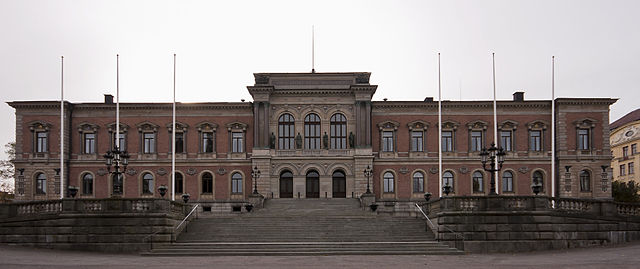
\includegraphics[width=400px]{images/universitetshuset} 

}

\caption{Universitetshuset}\label{fig:figureUniversitetshuset}
\end{figure}
\hypertarget{sec:resultat}{%
\section{Resultat}\label{sec:resultat}}
\begin{itemize}
\item
  Organize material and present results.
\item
  Use tables, figures (but prefer visual presentation):
  \begin{itemize}
  \item
    Tables and figures should supplement (and not duplicate) the text.
  \item
    Tables and figures should be provided with legends.
  \item
    \emph{Figure \ref{fig:graph} shows how to include and reference graphics.
    The graphic must be labelled before. Files must be in \textbf{.eps} format. You
    can do this really easily in R Markdown with \texttt{knitr::include\_graphics()}}!
  \item
    Figures can be referenced with \texttt{\textbackslash{}@ref(fig:\textless{}name\textgreater{})}, where \texttt{\textless{}name\textgreater{}} is the
    name of the code chunk.
  \end{itemize}
\end{itemize}
\begin{figure}

{\centering 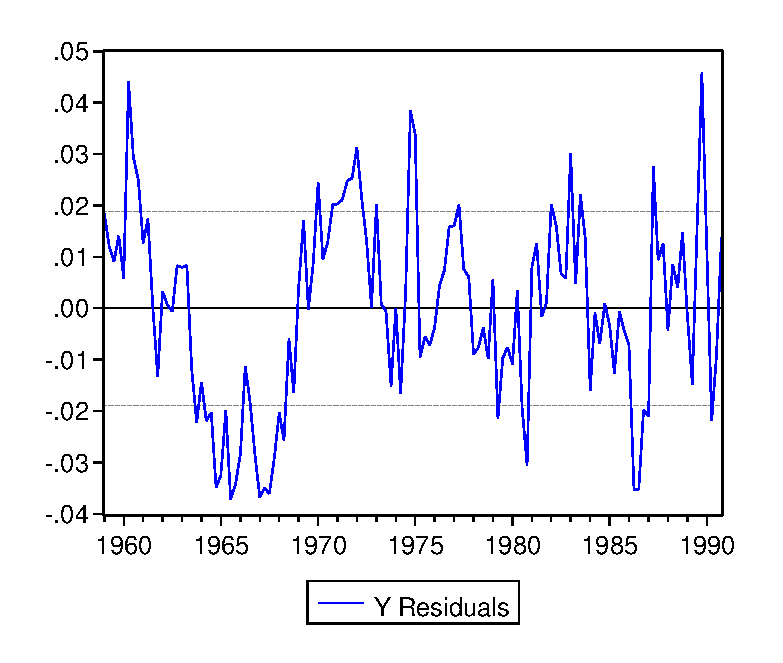
\includegraphics[width=0.5\linewidth]{figures/graph} 

}

\caption{Estimated residuals from model XXX. ...}\label{fig:graph}
\end{figure}
\begin{itemize}
\item
  Tables and graphics may appear in the text or in the appendix, especially if
  there are many simulation results tabulated, but is also depends on the study
  and number of tables resp. figures. The key graphs and tables must appear in
  the text!
\item
  R Markdown can also supports math equations just like \emph{LaTeX}!
  \begin{itemize}
  \item
    \emph{Equation \eqref{eq:SpecDens} represents the ACs of a stationary
    stochastic process:}
    \begin{equation}
            f_y(\lambda) = (2\pi)^{-1} \sum_{j=-\infty}^{\infty}
                           \gamma_j e^{-i\lambda j}
                         =(2\pi)^{-1}\left(\gamma_0 + 2 \sum_{j=1}^{\infty}
        \gamma_j \cos(\lambda j)\right)
                                       \label{eq:SpecDens}
    \end{equation}
    \emph{where \(i=\sqrt{-1}\) is the imaginary unit, \(\lambda \in [-\pi, \pi]\) is the
    frequency and the \(\gamma_j\) are the autocovariances of \(y_t\).}
  \item
    Equations can be referenced with \texttt{\textbackslash{}@ref(eq:\textless{}name\textgreater{})}, where name is defined
    by adding \texttt{(\textbackslash{}\#eq:\textless{}name\textgreater{})} in the line immediately before \texttt{\textbackslash{}end\{equation\}}.
  \end{itemize}
\end{itemize}
\hypertarget{review-of-results}{%
\subsection{Review of Results}\label{review-of-results}}
\begin{itemize}
\item
  Do the results support or do they contradict theory ?
\item
  What does the reader learn from the results?
\item
  Try to give an intuition for your results.
\item
  Provide robustness checks.
\item
  Compare to previous research.
\end{itemize}
\hypertarget{sec:slutsats}{%
\section{Slutsatser}\label{sec:slutsats}}
\begin{itemize}
\item
  Give a short summary of what has been done and what has been found.
\item
  Expose results concisely.
\item
  Draw conclusions about the problem studied. What are the implications of your
  findings?
\item
  Point out some limitations of study (assist reader in judging validity of
  findings).
\item
  Suggest issues for future research.
\end{itemize}
\newpage

\hypertarget{kuxe4llfuxf6rteckning}{%
\section*{Källförteckning}\label{kuxe4llfuxf6rteckning}}
\addcontentsline{toc}{section}{Källförteckning}

\noindent

\setlength{\parindent}{-0.5cm}
\setlength{\leftskip}{0.5cm}
\setlength{\parskip}{8pt}

\hypertarget{refs}{}
\begin{CSLReferences}{0}{0}
\leavevmode\vadjust pre{\hypertarget{ref-kuncheva2004combining}{}}%
Kuncheva, L. I. (2004) \emph{Combining pattern classifiers: Methods and algorithms}. John Wiley \& Sons.

\leavevmode\vadjust pre{\hypertarget{ref-lingenfelser2011systematic}{}}%
Lingenfelser, F., Wagner, J. and André, E. (2011) {`A systematic discussion of fusion techniques for multi-modal affect recognition tasks'}, in \emph{Proceedings of the 13th international conference on multimodal interfaces}. ACM, pp. 19--26.

\end{CSLReferences}
\indent
\setlength{\parindent}{17pt}
\setlength{\leftskip}{0pt}
\setlength{\parskip}{0pt}

\newpage

\appendix

\hypertarget{bilaga}{%
\section{Bilaga}\label{bilaga}}

Here goes the appendix!

\hypertarget{figurer}{%
\subsection{Figurer}\label{figurer}}
\begin{figure}

{\centering 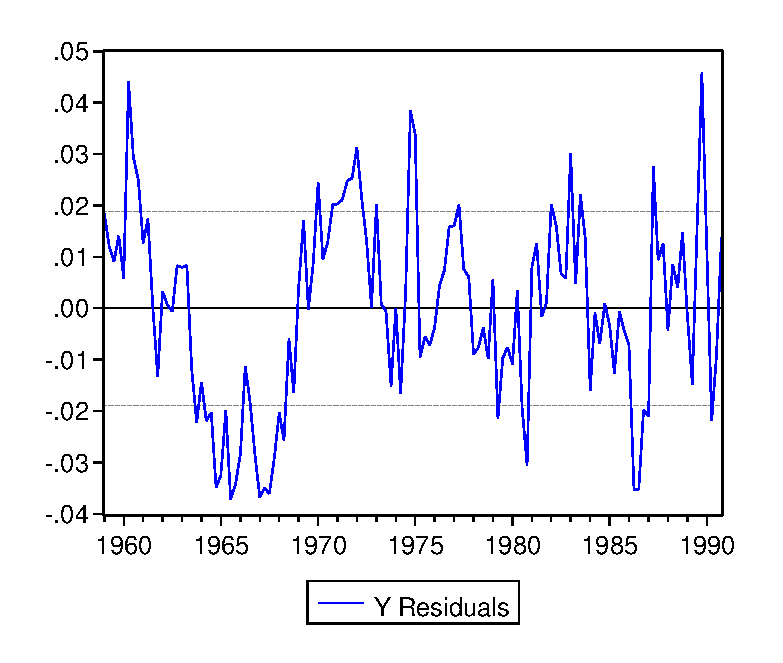
\includegraphics[width=0.5\linewidth,]{figures/graph} 

}

\caption{Estimated residuals (2) from model XXX. ...}\label{fig:graph2}
\end{figure}
\hypertarget{tabeller}{%
\subsection{Tabeller}\label{tabeller}}
\begin{table}[ht]
    \begin{center}
        {\footnotesize
        \begin{tabular}{l|cccccccccc}
        \hline \hline
                        & 3m    & 6m    & 1yr   & 2yr   & 3yr   & 5yr   & 7yr   & 10yr  & 12yr  & 15yr   \\
            \hline
                Mean   & 3.138 & 3.191 & 3.307 & 3.544 & 3.756 & 4.093 & 4.354 & 4.621 & 4.741 & 4.878  \\
                Median & 3.013 & 3.109 & 3.228 & 3.490 & 3.680 & 3.906 & 4.117 & 4.420 & 4.575 & 4.759  \\
                Min    & 1.984 & 1.950 & 1.956 & 2.010 & 2.240 & 2.615 & 2.850 & 3.120 & 3.250 & 3.395  \\
                Max    & 5.211 & 5.274 & 5.415 & 5.583 & 5.698 & 5.805 & 5.900 & 6.031 & 6.150 & 6.295  \\
                StD    & 0.915 & 0.919 & 0.935 & 0.910 & 0.876 & 0.825 & 0.803 & 0.776 & 0.768 & 0.762  \\
            \hline \hline
        \end{tabular}}
    \end{center}
    \caption{Detailed descriptive statistics of location and dispersion for
    2100 observed swap rates for the period from
    February 15, 1999 to March 2, 2007. Swap rates measured as 3.12 (instead of 0.0312).}
    \label{tab:apptable}
\end{table}
\newpage

% change rmd_files in `_bookdown.yml` files to determine order
% note that references and appendix are also contained here.


\end{document}
